\section{Introduction}
\def\R{\mathbb{R}}
\def\Z{\mathbb{Z}}

\begin{frame}
\frametitle{Discrete Time System}
For each time step $k \in \Z$ the system has:
\begin{itemize}
	\item A vector of input $u[k]$
	\item A vector of output $y[k]$
	\item A vector of states $x[k]$

\end{itemize}
\begin{figure}
	\centering
	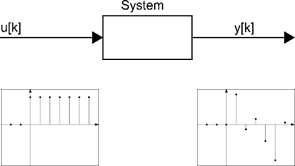
\includegraphics{Images/discrete_time_systems_1}
	\caption[An example of a discrete time system]{}
	\caption{}
	\label{fig:discrete_time_systems_1}
\end{figure}
\end{frame}

\begin{frame}
\frametitle{How to represent a system?}
\begin{itemize}
	\item Block-diagram
	\item State space representation
	\item Difference/differential equation
	\item Impulse response
	\item Transferfunctions
\end{itemize}

\end{frame}
\section{Block-diagram}
\begin{frame}
\frametitle{Block diagram}
\begin{figure}
\centering
\label{fig:discrete_time_systems_2}
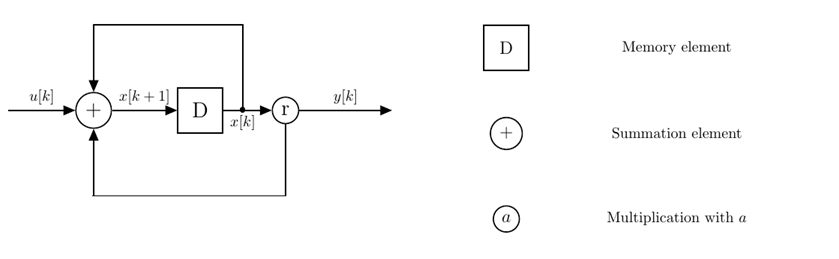
\includegraphics[width=0.8\linewidth]{Images/discrete_time_systems_2}
\caption{An example of a discrete time system}
\end{figure}
A block diagram is a visual representation of a system. All LTI’s (Linear Time Invariant) systems can be constructed using these 3 building blocks(Memory element, summation element, multiplication element). Note that every memory element corresponds to one state variable.
\end{frame}
\begin{frame}
	\frametitle{Example: compond interes}
	$ u[k]$:The deposits and withdrawals from the bank account
	$ x[k]$:The current saldo on bank account(before deposit and interest)
	$ y[k]$: The acquired interest of that year
	$ x[k+1]$: The saldo on the next year = current saldo + interest + deposits
	\begin{figure}
\centering
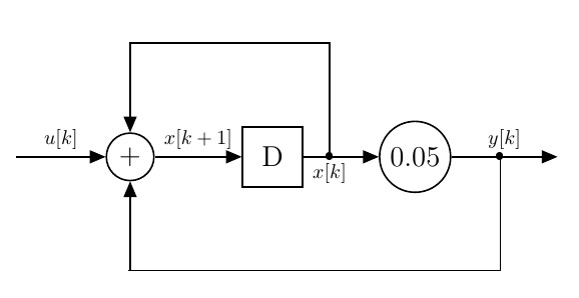
\includegraphics{Images/discrete_time_systems_3}
\caption{An example of compound interest with 5\% interest}
\label{fig:discrete_time_systems_3}
\end{figure}
\end{frame}
\begin{frame}
	\begin{tabular}{|c|c|c|c|}
		\hline  $u[k]$& $x[k+1]$  & $x[k]$  & $y[k]$  \\ 
		\hline  50 & 50 & 0  & 0  \\ 
		\hline  0 & 52.5  & 50 & 2.5  \\ 
		\hline  -25 & 30.13 & 52.5 & 2.62  \\ 
		\hline  0 &  31.63 & 30.13  & 1.51  \\ 
		\hline  0 & 33.21  & 31.63 & 1.58 \\ 
		\hline  30 & 64.87 & 33.21  & 1.66 \\ 
		\hline  0 & 68.12 & 64.87 & 3.24  \\ 
		\hline  0 & 71.52 & 68.12 & 3.41 \\
		\hline 
	\end{tabular}
	

\end{frame}
\begin{frame}
	\frametitle{Bad block diagrams}
	
		Delay-free loops:
		Delay-free loop:
		The issue is that this leads to an implicit connection 
		$u[k]$ depends on $y[k]$ ,which is not yet known
		You can easily rewrite this in an allowd shape
		$y[k] = u[k]  + 3 y[k] \Longleftrightarrow y[k] = -\frac{1}{2} u[k]$
		
\begin{figure}
\centering
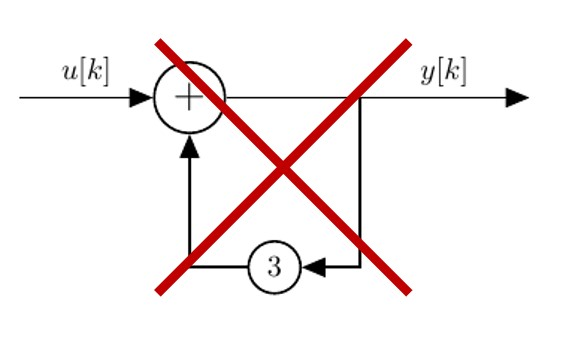
\includegraphics[width=5cm, height=3cm]{Images/discrete_time_systems_4}
\caption{An example of a delay free loop}
\label{fig:discrete_time_systems_4}
\end{figure}
\end{frame}
\begin{frame}
Connecting two outputs without using a sum: The issue is that this can lead to inconsistencies
According to this block diagram the output of the systems S1 and S2 are equal
There is no way to get around this.

\begin{figure}
\centering
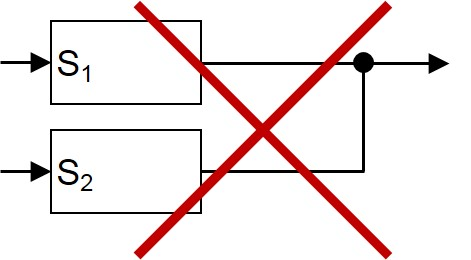
\includegraphics[width=5cm, height=3cm]{Images/discrete_time_systems_5}
\caption{}
\label{fig:discrete_time_systems_5}
\end{figure}
\end{frame}
\section{State Space representation}
\begin{frame}
	\frametitle{State space representation}
	\begin{center}
	$x[k+1] = A x[k] + B u[k]$ \\
	$y[k] = C x[k] + D u[k] $ \\
	\end{center}
	This state space representation is again specific to LTI systems:
	Linear: it’s easy to see these systems are linear (see lecture about classification of dynamical systems)
	Time-invariant: the matrices A,B,C,D do not depend on time, if it were to be a time-variant system the matrices would be replaced by $A[k], B[k], C[k] and D[k]$. \\
\end{frame}
\begin{frame}
\frametitle{From block diagram to state space }
\begin{columns}

\begin{column}{0.5\textwidth}

	Blockdiagram:
	\begin{figure}
\centering
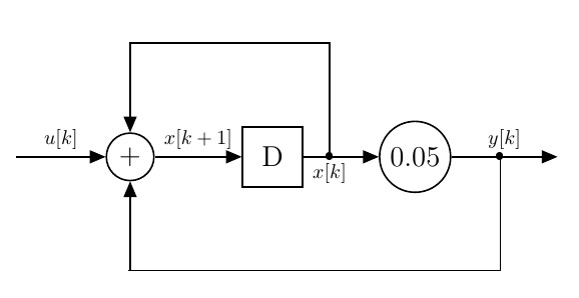
\includegraphics[width=1\linewidth]{Images/discrete_time_systems_3}
\caption{}
\label{fig:discrete_time_systems_3}
\end{figure}
\end{column}
\begin{column}{0.5\textwidth}
	State space representation: \\
	In general
	Let the inputs of the memory element be	and the outputs	.
	Trace back to retrieve equations for $x_i[k+1] $   and $y_i[k]$ 
	This results in:
	\begin{center}
	$x[k+1] = u[k] + 1.05 x[k] $
	$y[k] = 0.05 x[k]$
	\end{center}
	
\end{column}
\end{columns}
\end{frame}
\begin{frame}
	\frametitle{From state space to block diagram (DT)}
		\begin{center}
			$x[k+1] = A x[k] + B u[k]$ \\
			$y[k] = C x[k] + D u[k] $ \\

	with  A = 
	$\begin{bmatrix}
		1 & 0 & 0 \\
		0 & 0 & 1 \\
		0 & 3 & 0
	\end{bmatrix}$, B = $\begin{bmatrix}
	1\\
	0\\
	4\\
\end{bmatrix}$, C = $\begin{bmatrix}
 5 & 1 & 0
\end{bmatrix}$ and D = $\begin{bmatrix}
1
\end{bmatrix}$ \\
\end{center}
	First add a delay element for every state $x_i[k]$


\end{frame}
\begin{frame}
	\frametitle{From state space to block diagram (DT)}
	Add a delay element for every state x[k]
	Determine the input for every state x[k+1] from the matrixes A and B, as a combination of the states x[k] and inputs u[k]
	
\end{frame}
\begin{frame}
	\frametitle{Different state space representations}
	State space representation is not unique:
	Take the following system, which connects u[k] to y[k]:
		\begin{center}
			$x[k+1] = A x[k] + B u[k]$ \\
			$y[k] = C x[k] + D u[k] $ \\
		\end{center}
	Now take a non-singular square matrix T and the following system. The relation between u[k] and y[k] will be the same.
	\begin{center}
		$Tx[k+1] = TAT^{-1}Tx[k] + TBu[k]\\
		y[k] = C T^{-1}Tx[k] + Du[k]$
	\end{center}
	With $x' = Tx, A' = TAT^{-1},B' = TB,C' = CT^{-1}$ and $D'=D$	,  we have found a different state space representation for this system.
	The same holds for continuous time.
	
\end{frame}
\begin{frame}
	\frametitle{Different state space representations}
	Input-output behavior is maintained
	Internal behavior can be very different
	If A has an Eigenvalue decomposition PDP-1 and T = P-1 then the resulting state space model will be greatly simplified
	If no Eigenvalue decomposition exists for A then a Jordan form may be used.
	
\end{frame}
\section{Diffence equations}
\begin{frame}
	\frametitle{Diffence equations}
	Similar to differential equations, but for discrete time
	General form: $\sum\limits_{i=0}^n a_iy[k+i] = \sum\limits_{i=0}^n b_iu[k+i]$
	n is the order of the system
	k is usually taken to be larger than zero
	Each value y[k+i] represents the output of the system at a moment k+i
	Each value u[k+i] represents an external input delivered to the system
	Solution in 2 parts:
	homogenous: solution from input zero
	particular: solution derived as a response from the input
\end{frame}
\begin{frame}
	\frametitle{Homogenous difference equations}
	General form: $\sum\limits_{i=0}^n a_iy[k+i]= 0$ \\
	e.g. : $5y[k+1] - y[k] = 0
	y[k+1] = \frac{1}{5}y[k] \\
	y[1] = \frac{1}{5} y[0] \\
	y[2] = \frac{1}{5}y[1] = (\frac{1}{5})^2y[0]\\
	\vdots
	y[n] = (\frac{1}{5})^{n}y[0]$
	Expected form of solution: $r^{k}$
	Substitution of the expected solution in the difference equation:
	$\sum\limits_{i=0}^n a_ir^{k+i}= 0$
	Division by rk leads to the characteristic equation:
	$\sum\limits_{i=0}^n a_ir^{i}= 0$
	Solutions of the characteristic equation:
	$r_1,r_2,r_3$
	Homogenous solution to the difference equation: 
	$y[k] = c_1r_1^{k} + c_2r_2^{k} + c_3r_3^{k} + \cdots$
	
	
\end{frame}
